\section{Solver Options}
\label{sec:solver_options}

The Solver Options tab contains settings defining exactly how a given problem should run. \ac{EMTG} contains both a local gradient-based optimizer and a stochastic global search heuristic called (\ac{MBH}), each with various options which may be modified as needed. Users may choose run the local optimizer and the stochastic search heuristic together, the local optimizer alone, or instead just evaluate a set of controls as an initial guess. 

\begin{figure}[H]
    \centering
    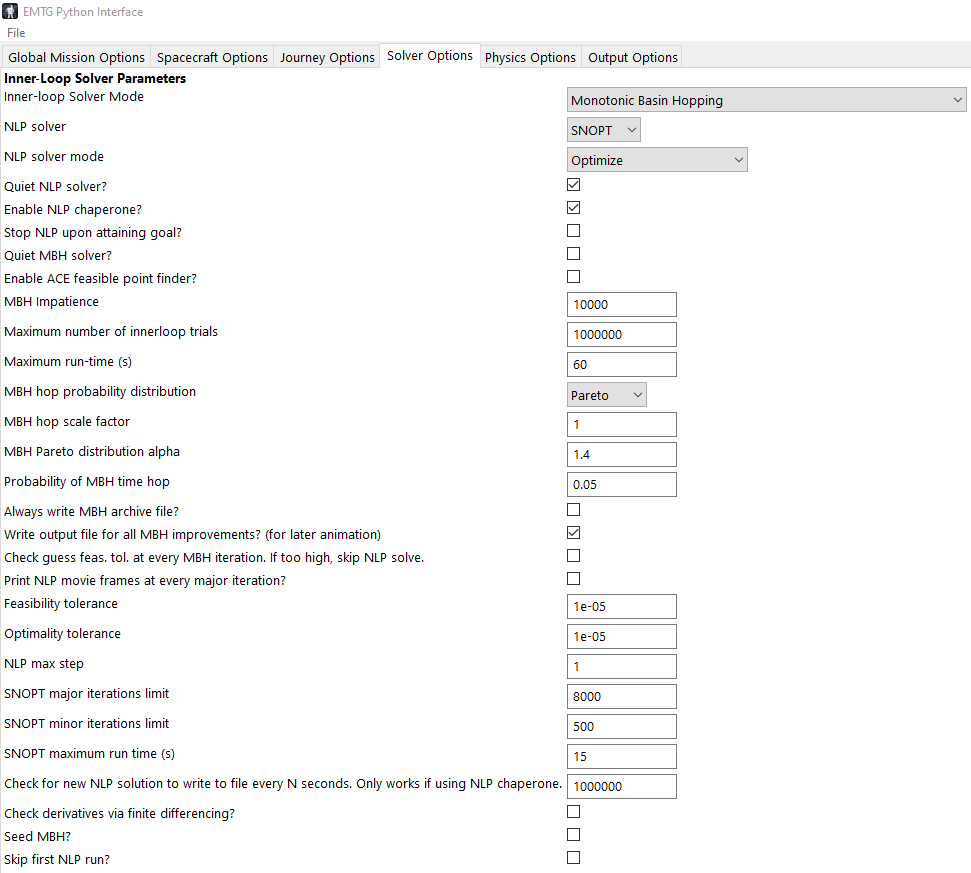
\includegraphics[width=1.0\textwidth]{../../shared_latex_inputs/images/pyemtg_solver_options_tab.png}
    \caption{EMTG Solver Options tab}
\end{figure}

\noindent Users may choose which solver mode to use via the \textbf{Inner-loop Solver Mode} option: \\
\begin{table}[H]
    \hspace{2cm}
    \begin{tabular}{lp{5cm}}
    \ac{EMTG} Variable Name & \verb|run_inner_loop| \\
    Data Type & \verb|(InnerLoopSolverType) enum| \\
    Allowed Values & \verb|0: None, evaluate trialX| \newline
                    \verb|1: Monotonic Basin Hopping,| \newline
                    \verb|2: Adaptive Constrained DE (NOT IMPLEMENTED),| \newline
                    \verb|3: NLP with initial guess,| \newline
                    \verb|4: Filament walker (experimental)| \\
    Default Value & \verb|1: Monotonic Basin Hopping| \\
    \end{tabular}
\end{table}


\listitem{Evaluate trialX}{Propagate an initial guess without solving. This will user either the Keplerian propagator or integrate the equations of motion, depending on the users chosen mission type and physics settings. Users must provide an initial guess as a {\tt .emtg} solution file via the ``Trial decision vector or initial guess'' input option.}
\indent\listitem{\ac{NLP} with initial guess}{Leverages a gradient-based solver to solve a problem given an initial guess. Currently, the only available solver is the \ac{SNOPT}. More detail is provided in \ref{sec:gradient_based_solver}. Users must provide an initial guess as a {\tt .emtg} solution file via the ``Trial decision vector or initial guess'' input option.}
\indent\listitem{Monotonic Basin Hopping}{This solver mode allows users to provide no initial guess and instead generate one with the \ac{MBH} stochastic global search method. This runs in conjunction with the gradient-based solver to allow users to start with no initial guess and obtain a satisfied, locally optimized solution. In theory, if users allow \ac{MBH} to run for extended periods of time, this will ensure solutions converge to globally or near-globally optimal solutions. More detail is provided in \ref{sec:monotonic_basin_hopping}.}

\subsection{Gradient-Based Solver}
\label{sec:gradient_based_solver}
The optimization problems in \ac{EMTG} are formulated as Nonlinear Programming (\ac{NLP}) problems. Thus, the optimizer solves a problem of the form: \\
\begingroup
\addtolength{\jot}{-2pt}
\begin{flalign*}
    &\textrm{Minimize} f(\mathbf{x}) \\
    &\textrm{Subject to:} \\
    &\mathbf{x}_{lb} \leq \mathbf{x} \leq \mathbf{x}_{ub} \\
    &\mathbf{c(x)} \leq \mathbf{0} \\
    &A \cdot \mathbf{x} \leq 0
\end{flalign*}
\endgroup
\noindent where $\mathbf{x}_{lb}$ and $\mathbf{x}_{ub}$ define the lower and upper bounds on the decision (control) vector, $\mathbf{c(x)}$ is a vector of nonlinear constraint functions, and $A$ is a matrix describing linear constraints.

\noindent Since most interplanetary trajectory optimization problems may consist of hundreds of variables and tens to hundreds of constraints, these problems are best solved with sparse \ac{NLP} solvers. \ac{EMTG} leverages the \ac{SNOPT} to solve these problems. For detailed information on this optimizer beyond what is described here, see the \ac{SNOPT} user guide at \href{https://web.stanford.edu/group/SOL/guides/sndoc7.pdf}{https://web.stanford.edu/group/SOL/guides/sndoc7.pdf}.

\noindent \ac{SNOPT} uses a sparse sequential quadratic programming (SQP) method and benefits greatly from partial derivatives with respect to the decision variables. \ac{EMTG} is designed to provide analytical expressions for all necessary partial derivatives (objectives and constraints) which improves convergence. Users may modify the following options for the \ac{NLP} solver: \\


\begin{enumerate}

    \item \textbf{\ac{NLP} solver:} Allows users to choose which of the available \ac{NLP} solvers to use. Currently, only \ac{SNOPT} may be used.
        \begin{table}[H]
            \hspace{2cm}
            \begin{tabular}{lp{5cm}}
            \ac{EMTG} Variable Name & \verb|NLP_solver_type| \\
            Data Type & \verb|int| \\
            Allowed Values & \verb|0: \ac{SNOPT},| \newline
                            \verb|1: WORHP|  \\
            Default Value & \verb|0: \ac{SNOPT}| \\
            \end{tabular}
        \end{table}

    \item \textbf{\ac{NLP} solver mode:} Sets the \ac{NLP} solver to solve the problem in various ways, such as finding a solution which only satisfies equality constraints, finding a solution which is feasible, and finding a feasible solution and minimizing or maximizing the chosen objective.
        \begin{table}[H]
            \hspace{2cm}
            \begin{tabular}{lp{5cm}}
            \ac{EMTG} Variable Name & \verb|NLP_solver_mode| \\
            Data Type & \verb|(NLPMode) enum| \\
            Allowed Values & \verb|0: Feasible point,| \newline
                            \verb|1: Optimize,| \newline
                            \verb|2: Satisfy equality constraints| \\
            Default Value & \verb|1: Optimize| \\
            \end{tabular}
        \end{table}
    
    \item \textbf{Quiet \ac{NLP} solver?:} Sets whether the \ac{NLP} solver should be quiet such that iterations are not displayed in the \ac{EMTG} terminal.
        \begin{table}[H]
            \hspace{2cm}
            \begin{tabular}{lp{5cm}}
            \ac{EMTG} Variable Name & \verb|quiet_NLP| \\
            Data Type & \verb|bool| \\
            Allowed Values & true, false \\
            Default Value & true \\
            \end{tabular}
        \end{table}

    \item \textbf{Enable \ac{NLP} chaperone?:}{Allows \ac{EMTG} to recover the best solution found in a run of \ac{SNOPT} even if \ac{SNOPT} does not converge. It is recommended to turn this setting on in most cases.}
        \begin{table}[H]
            \hspace{2cm}
            \begin{tabular}{lp{5cm}}
            \ac{EMTG} Variable Name & \verb|enable_NLP_chaperone| \\
            Data Type & \verb|bool| \\
            Allowed Values & true, false \\
            Default Value & true \\
            \end{tabular}
        \end{table}

    \item \textbf{Stop \ac{NLP} upon attaining goal?:} Option to force \ac{NLP} solver to stop once a desired objective goal is satisfied, even if the optimizer may be able to minimize further.
        \begin{table}[H]
            \hspace{2cm}
            \begin{tabular}{lp{5cm}}
            \ac{EMTG} Variable Name & \verb|NLP_stop_on_goal_attain| \\
            Data Type & \verb|bool| \\
            Allowed Values & true, false \\
            Default Value & false \\
            \end{tabular}
        \end{table}

    \item \textbf{\ac{NLP} objective goal:} User specified numeric objective value used to define the ``Stop \ac{NLP} upon attaining goal'' option criteria. This is set as an unscaled value. In PyEMTG, this option only appears after selecting the ``Stop \ac{NLP} upon attaining goal'' option.
        \begin{table}[H]
            \hspace{2cm}
            \begin{tabular}{lp{5cm}}
            \ac{EMTG} Variable Name & \verb|NLP_objective_goal| \\
            Data Type & \verb|double| \\
            Default Value & 0 \\
            Units & various
            \end{tabular}
        \end{table}

    \item \textbf{Print \ac{NLP} movie frames at every major iteration?:} Option to print \ac{NLP} information at each major iteration, including constraints descriptions and bounds. This will generate ``\ac{NLP}\_Frame\_\#.csv'' files containing the variable being constrained, the constraint lower and upper bounds, the scale factor for the constraint, and the actual value of the variable.
        \begin{table}[H]
            \hspace{2cm}
            \begin{tabular}{lp{5cm}}
            \ac{EMTG} Variable Name & \verb|print_NLP_movie_frames| \\
            Data Type & \verb|bool| \\
            Allowed Values & true, false \\
            Default Value & false \\
            \end{tabular}
        \end{table}

    \item \textbf{Feasibility tolerance:} Tolerance for defining feasibility of a solution with respect to provided constraints. This is described in further detail in the \ac{SNOPT} user guide.
    \begin{table}[H]
        \hspace{2cm}
        \begin{tabular}{lp{5cm}}
        \ac{EMTG} Variable Name & \verb|snopt_feasibility_tolerance| \\
        Data Type & \verb|double| \\
        Allowed Values & $-\infty$ $<$ Real $<$ $\infty$ \\
        Default Value & 1E-5 \\
        Units & various
        \end{tabular}
    \end{table}
    
    \item \textbf{Optimality tolerance:} Tolerance for defining optimality of a solution. This is described in further detail in the \ac{SNOPT} user guide.
    \begin{table}[H]
        \hspace{2cm}
        \begin{tabular}{lp{5cm}}
        \ac{EMTG} Variable Name & \verb|snopt_optimality_tolerance| \\
        Data Type & \verb|double| \\
        Allowed Values & $-\infty$ $<$ Real $<$ $\infty$ \\
        Default Value & 1E-5 \\
        Units & various
        \end{tabular}
    \end{table}
    
    \item \textbf{\ac{NLP} max step:} Sets the maximum step size during a linesearch in \ac{SNOPT}.
    \begin{table}[H]
        \hspace{2cm}
        \begin{tabular}{lp{5cm}}
        \ac{EMTG} Variable Name & \verb|NLP_max_step| \\
        Data Type & \verb|double| \\
        Allowed Values & $0$ $<$ Real $<$ $\infty$ \\
        Default Value & $1$ \\
        Units & various
        \end{tabular}
    \end{table}
    
    \item \textbf{\ac{SNOPT} major iterations limit:} Sets the maximum number of major iterations \ac{SNOPT} may perform. This defines how many times the quadratic subproblem will be solved when optimizing an objective.
    \begin{table}[H]
        \hspace{2cm}
        \begin{tabular}{lp{5cm}}
        \ac{EMTG} Variable Name & \verb|snopt_major_iterations| \\
        Data Type & \verb|size_t| \\
        Allowed Values & $0$ $<$ Real $<$ $\infty$ \\
        Default Value & $8000$ \\
        \end{tabular}
    \end{table}
    
    \item \textbf{\ac{SNOPT} minor iterations limit:} Sets the maximum number of minor iterations \ac{SNOPT} may perform. This defines the number of iterations allowed in solving each quadratic subproblem for each major iteration.
    \begin{table}[H]
        \hspace{2cm}
        \begin{tabular}{lp{5cm}}
        \ac{EMTG} Variable Name & \verb|snopt_minor_iterations| \\
        Data Type & \verb|size_t| \\
        Allowed Values & $0$ $<$ Real $<$ $\infty$ \\
        Default Value & $500$ \\
        \end{tabular}
    \end{table}
    
    \item \textbf{\ac{SNOPT} maximum run time:} The maximum amount of time allowed for any \ac{SNOPT} run.
    \begin{table}[H]
        \hspace{2cm}
        \begin{tabular}{lp{5cm}}
        \ac{EMTG} Variable Name & \verb|snopt_max_run_time| \\
        Data Type & \verb|int| \\
        Allowed Values & $0$ $<$ Real $<$ $\infty$ \\
        Default Value & $15$ \\
        Units & seconds
        \end{tabular}
    \end{table}
    
    \item \textbf{Check for new \ac{NLP} solution to write to file every N seconds. Only works if using \ac{NLP} chaperone.:} When using the \ac{NLP} chaperone, sets the number of seconds between checking for a new intermediate \ac{NLP} solution. New intermediate \ac{NLP} solutions are written to the file.
    \begin{table}[H]
        \hspace{2cm}
        \begin{tabular}{lp{5cm}}
        \ac{EMTG} Variable Name & \verb|print_NLP_movie_frames| \\
        Data Type & \verb|bool| \\
        Allowed Values & true, false \\
        Default Value & false \\
        \end{tabular}
    \end{table}
    
    
    \item \textbf{Check derivatives via finite differencing?:} Option to tell \ac{SNOPT} to check the derivatives by verifying both the individual gradients and the individual columns of the Jacobian are satisfactory.
    \begin{table}[H]
        \hspace{2cm}
        \begin{tabular}{lp{5cm}}
        \ac{EMTG} Variable Name & \verb|check_derivatives| \\
        Data Type & \verb|bool| \\
        Allowed Values & true, false \\
        Default Value & false \\
        \end{tabular}
    \end{table}
    
    \item \textbf{Trial decision vector or initial guess:} Option to select a previous {\tt .emtg} solution file as an initial guess for another run, even if some aspects of the problem have changed (e.g., increasing fidelity by changing the Mission Type, see Chapter \ref{chap:mission_types}). \ac{EMTG} has built in capability to handle differences between the current {\tt .emtgopt} file and the provided initial guess solution file. 

\end{enumerate}




\subsection{Monotonic Basin Hopping}
\label{sec:monotonic_basin_hopping}
(\ac{MBH}) is a stochastic global search heuristic which allows \ac{EMTG} to search for globally optimal solutions and run without an initial guess. This algorithm helps to find the best solutions in problems with many local optima. Often problems are structured such that individually local optimal ``basins'' cluster together, such that the distance in the decision space from one local optima to the next in a given cluster may be traversed in a short ``hop''. In \ac{EMTG}, the ``hop'' is calculated and applied using the scaled decision variables rather than the dimensional decision variables. Additional details on \ac{MBH}, including an algorithm detailing its process, may be found in in Section 15.3 of the \ac{EMTG} Software Design Document. A diagram detailing how \ac{MBH} may improve a solution for a problem with many local optima is shown in Figure \ref{fig:MBH}.

\noindent The version of \ac{MBH} in \ac{EMTG} has two major parameters which a user has control over: the stopping criterion, and the type of random step used to generated the perturbed decision vector. The stopping criterion is defined by providing a maximum number of trial points to attempt (which directly translates to iterations) or a maximum CPU run time. The type of random step is defined by a probability distribution and various parameters which describe that distribution. Typically, a Pareto distribution described by some Pareto parameter $\alpha$ is used. \ac{MBH} may be started from either a uniform-randomly chosen point in the decision space when not providing an initial guess or from an initial guess derived from a previous problem.


% Move this to the description of "Probability of MBH time hop." 
% In EMTG, special attention is given to decision variables that define time-of-flight between two boundary points. These are arguably the most significant variables defining a trajectory, and thus it is sometimes necessary to significantly perturb them in order to successfully ``hop'' to a new cluster of solutions. This is achieved via a low uniform-random probability which shifts the time-of-flight variables by $\pm$ 1 synodic period of the two boundary points.

\begin{figure}
	\centering
	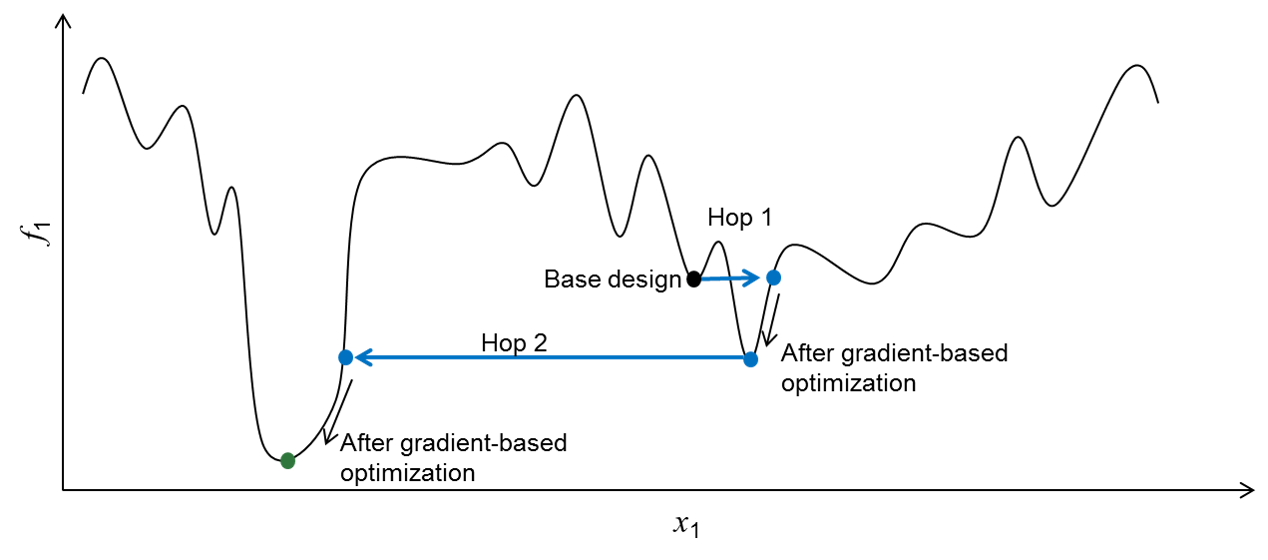
\includegraphics[width=0.8\linewidth]{../../shared_latex_inputs/images/MBH.png}
	\caption{Monotonic Basin Hopping on a 1-dimensional function.}
	\label{fig:MBH}
\end{figure}

\noindent Users may modify the following options for \ac{MBH} to suit their needs: \\

\begin{enumerate}
    \item \textbf{Enable ACE feasible point finder?:} Allows \ac{MBH} to compare infeasible solutions and search for minimum infeasibility before finding the first feasible solution. The most feasible of the infeasible solutions is then used as the next initial trial point before further hop perturbations are applied, which helps \ac{MBH} continuously improve its solutions prior to obtaining a feasible solution. This runs prior to \ac{SNOPT} if the initial feasibility is larger than the user specified constraint set for skipping the \ac{NLP} solve, and after \ac{SNOPT} every iteration until a point satisfying the \ac{SNOPT} feasibility tolerance is satisfied.
    \begin{table}[H]
        \hspace{2cm}
        \begin{tabular}{lp{5cm}}
        \ac{EMTG} Variable Name & \verb|ACE_feasible_point_finder| \\
        Data Type & \verb|bool| \\
        Allowed Values & true, false \\
        Default Value & false \\
        \end{tabular}
    \end{table}
    
    \item \textbf{\ac{MBH} Impatience:} Defines the number of \ac{MBH} perturbations to try near the current feasible point before obtaining a new random point. If this number of trials is reached, \ac{MBH} returns a new random point before performing further perturbations.
    \begin{table}[H]
        \hspace{2cm}
        \begin{tabular}{lp{5cm}}
        \ac{EMTG} Variable Name & \verb|MBH_max_not_improve| \\
        Data Type & \verb|int| \\
        Allowed Values & $0$ $<$ Real $<$ $\infty$ \\
        Default Value & 1E4 \\
        \end{tabular}
    \end{table}
    
    \item \textbf{\ac{MBH} Impatience when skipping \ac{NLP} Solve:} Defines the number of \ac{MBH} perturbations to continue trying near the current feasible point before obtaining a new random point when skipping \ac{NLP} solve due to not satisfying the guess feasibility tolerance requirement. If this number of trials is reached, \ac{MBH} returns a new random point before performing further perturbations. Hidden until the ``Check guess feas. tol.'' option is selected.
    \begin{table}[H]
        \hspace{2cm}
        \begin{tabular}{lp{5cm}}
        \ac{EMTG} Variable Name & \verb|MBH_max_not_improve_with_NLP_skip| \\
        Data Type & \verb|int| \\
        Allowed Values & $0$ $<$ Real $<$ $\infty$ \\
        Default Value & 1E4 \\
        \end{tabular}
    \end{table}
    
    
    \item \textbf{Maximum number of innerloop trials:} Sets the maximum number of \ac{MBH} trials to run before returning the best feasible point found.
    \begin{table}[H]
        \hspace{2cm}
        \begin{tabular}{lp{5cm}}
        \ac{EMTG} Variable Name & \verb|MBH_max_trials| \\
        Data Type & \verb|int| \\
        Allowed Values & $0$ $<$ Real $<$ $\infty$ \\
        Default Value & 1E6 \\
        \end{tabular}
    \end{table}
    
    \item \textbf{Maximum run-time (s):} Sets the maximum CPU run time of \ac{MBH} before returning the best feasible point found.
    \begin{table}[H]
        \hspace{2cm}
        \begin{tabular}{lp{5cm}}
        \ac{EMTG} Variable Name & \verb|MBH_max_run_time| \\
        Data Type & \verb|int| \\
        Allowed Values & $0$ $<$ Real $<$ $\infty$ \\
        Default Value & $60$ \\
        \end{tabular}
    \end{table}
    
    \item \textbf{\ac{MBH} hop probability distribution:} Allows a user to choose between ``Uniform'', ``Cauchy'', ``Pareto'', or ``Gaussian'' probability distributions to randomly calculate the step size for a hop perturbation. These options have various additional parameters to help define the distribution.
    \begin{table}[H]
        \hspace{2cm}
        \begin{tabular}{lp{5cm}}
        \ac{EMTG} Variable Name & \verb|MBH_hop_distribution| \\
        Data Type & \verb|int| \\
        Allowed Values & \verb|0: Uniform,| \newline
                        \verb|1: Cauchy,| \newline
                        \verb|2: Pareto,| \newline
                        \verb|3: Gaussian| \\
        Default Value & \verb|2: Pareto| \\
        \end{tabular}
    \end{table}
    
    \item \textbf{\ac{MBH} uniform hop ball size:} For the ``Uniform'' probability distribution, this scales the randomly generated perturbation on the decision variables, i.e. increases the size of the uniform ``ball'' used to generate the perturbations.
    \begin{table}[H]
        \hspace{2cm}
        \begin{tabular}{lp{5cm}}
        \ac{EMTG} Variable Name & \verb|MBH_max_step_size| \\
        Data Type & \verb|double| \\
        Allowed Values & $0$ $<$ Real $<$ $\infty$ \\
        Default Value & $1$ \\
        \end{tabular}
    \end{table}
    
    \item \textbf{\ac{MBH} hop scale factor:} For the ``Cauchy'' and ``Pareto'' probability distributions, this scales the randomly generated perturbation on the decision variables.
    \begin{table}[H]
        \hspace{2cm}
        \begin{tabular}{lp{5cm}}
        \ac{EMTG} Variable Name & \verb|MBH_max_step_size| \\
        Data Type & \verb|double| \\
        Allowed Values & $0$ $<$ Real $<$ $\infty$ \\
        Default Value & $1$ \\
        \end{tabular}
    \end{table}
    
    \item \textbf{\ac{MBH} Pareto distribution alpha:} For the ``Pareto'' probability distribution, sets the Pareto parameter $\alpha$ to define how the random step is drawn from the bi-directional Pareto distribution.
    \begin{table}[H]
        \hspace{2cm}
        \begin{tabular}{lp{5cm}}
        \ac{EMTG} Variable Name & \verb|MBH_Pareto_alpha| \\
        Data Type & \verb|double| \\
        Allowed Values & $0$ $<$ Real $<$ $\infty$ \\
        Default Value & $1.4$ \\
        \end{tabular}
    \end{table}
    
    \item \textbf{\ac{MBH} hop standard deviation:} For the ``Gaussian'' probability distribution, this sets the standard deviation which defines the Gaussian distribution used to generate the perturbation for the decision variables.
    \begin{table}[H]
        \hspace{2cm}
        \begin{tabular}{lp{5cm}}
        \ac{EMTG} Variable Name & \verb|MBH_max_step_size| \\
        Data Type & \verb|double| \\
        Allowed Values & $0$ $<$ Real $<$ $\infty$ \\
        Default Value & $1$ \\
        \end{tabular}
    \end{table}
    
    \item \textbf{Probability of \ac{MBH} time hop:} Special attention is given to decision variables that define time-of-flight between two boundary points in the \ac{MBH} algorithm. These are the most significant variables defining an interplanetary trajectory, and thus it is sometimes necessary to significantly perturb them in order to successfully ``hop'' to a new cluster of solutions. This is achieved via a low uniform-random probability which shifts the time-of-flight variables by $\pm$ 1 synodic period of the two boundary points.
    \begin{table}[H]
        \hspace{2cm}
        \begin{tabular}{lp{5cm}}
        \ac{EMTG} Variable Name & \verb|MBH_time_hop_probability| \\
        Data Type & \verb|double| \\
        Allowed Values & $0$ $<$ Real $<$ $\infty$ \\
        Default Value & $0.05$ \\
        \end{tabular}
    \end{table}
    
    \item \textbf{Always write \ac{MBH} archive file?:} Option to choose whether to always save an archive file of the \ac{MBH} runs. An archive file has extension {\tt .emtg\_archive} and stores basic information from the \ac{MBH} runs, including the number of times the point was reset, the number of total iterations \ac{MBH} took, the time stamp in seconds of when an iteration of \ac{MBH} completed, and the objective function value of that iteration.
    \begin{table}[H]
        \hspace{2cm}
        \begin{tabular}{lp{5cm}}
        \ac{EMTG} Variable Name & \verb|MBH_always_write_archive| \\
        Data Type & \verb|bool| \\
        Allowed Values & true, false \\
        Default Value & false \\
        \end{tabular}
    \end{table}
    
    \item \textbf{Write output file for all \ac{MBH} improvements? (for later animation):} Option to print a ``hop'' data file for every \ac{MBH} improvement, which can then be used to animate the results of \ac{MBH}.
    \begin{table}[H]
        \hspace{2cm}
        \begin{tabular}{lp{5cm}}
        \ac{EMTG} Variable Name & \verb|MBH_write_every_improvement| \\
        Data Type & \verb|bool| \\
        Allowed Values & true, false \\
        Default Value & false \\
        \end{tabular}
    \end{table}
    
    \item \textbf{Check guess feas. tol. at every \ac{MBH} iteration. If too high, skip \ac{NLP} solve.:} Option to have \ac{MBH} check if a solution satisfies a user provided feasibility tolerance and skip the \ac{NLP} solve call in an \ac{MBH} trial run if the feasibility tolerance is not satisfied.
    \begin{table}[H]
        \hspace{2cm}
        \begin{tabular}{lp{5cm}}
        \ac{EMTG} Variable Name & \verb|checkFeasibilityTolInMBHToSkipNLP| \\
        Data Type & \verb|bool| \\
        Allowed Values & true, false \\
        Default Value & false \\
        \end{tabular}
    \end{table}
    
    \item \textbf{Skip \ac{NLP} solve if feas. tol. of initial guess is greater than this value. (\ac{MBH} only.):} Tolerance used to determine if the \ac{MBH} iteration returns a point that is acceptable enough to perform an \ac{NLP} solve. If the feasibility is worse than this provided tolerance, the \ac{NLP} solve is skipped and the next \ac{MBH} iteration begins. Hidden until the ``Check guess feas. tol.'' option is selected.
    \begin{table}[H]
        \hspace{2cm}
        \begin{tabular}{lp{5cm}}
        \ac{EMTG} Variable Name & \verb|feasibilityTolInMBHToSkipNLP| \\
        Data Type & \verb|double| \\
        Allowed Values & $-\infty$ $<$ Real $<$ $\infty$ \\
        Default Value & 1E6 \\
        \end{tabular}
    \end{table}
    
\end{enumerate}


